\documentclass[12pt]{report}
\title{R(D*) Analysis Guide and Thoughts}
\author{Anthony LaTorre}
\usepackage{hyperref}
\usepackage{caption}
\usepackage{listings}
\lstset{
  basicstyle=\ttfamily,
  columns=fullflexible,
  frame=none,
  breaklines=true,
  postbreak=\mbox{\textcolor{red}{$\hookrightarrow$}\space},
}
\usepackage{xcolor}
\usepackage[framemethod=TikZ]{mdframed}
\mdfsetup{nobreak=true}
\usepackage{fullpage}
\definecolor{light-gray}{gray}{0.95} %the shade of grey that stack exchange uses
\begin{document}
\maketitle
\tableofcontents
\begin{abstract}
This is a short document intended to provide an intro to the R(D*) analysis and
talk about some of the current problems. Currently there are many
disagreements between data and MC on very fundamental inputs to the analysis
(like covariance matrices and primary vertex track fits). I believe the current
approach of trying to fix upstream MC problems with downstream corrections for
these will not produce a reliable estimate of R(D*).
\end{abstract}
\chapter{Introduction}
This document is intended to give a brief overview of the technical details of
the software and some current problems with the R(D*) analysis. Before diving
in, you should read the following documents to help you get a better idea of
the overall analysis strategy:
\begin{itemize}
\item Analysis Note: \url{https://cms.cern.ch/iCMS/jsp/db_notes/noteInfo.jsp?cmsnoteid=CMS%20AN-2019/162}
\item Olmo's Thesis: \url{https://thesis.library.caltech.edu/15019/1/olmo_cerri_2023_thesis.pdf}
\end{itemize}
\section{History}
This analysis was created by Olmo Cerri during his PhD. I started working on
the analysis after it was at a very advanced stage (after an initial unblinding
that was reblinded). Olmo and I worked on trying to fix issues with the fit for
a year. During this period we made many improvements:
\begin{itemize}
\item added several new backgrounds
\item added effects to account for event migration between bins
\item try and correct for covariance matrix differences between data and MC
\item relax p-value cuts since p-values for the track fits never agreed between data and MC
\item investigate form factor pulling
\item + many more
\end{itemize}
and since he graduated I have added a few more improvements (PV smearing being
the most important).

\section{General Thoughts on the Analysis and comparison to LHCB}
I think the general approach to the analysis is very strong. The idea of doing
a full multi-dimensional likelihood fit with the control regions fit
simultaneously is a very good approach. The recent result from LHCB (see
\url{https://indico.cern.ch/event/1187939/attachments/2530158/4355180/DTaunu_CERNSeminar.pdf})
are very impressive in some respects but are not as rigorous as this analysis
in several others. The most impressive part of the analysis I thought is that
they did two independent analyses which agreed at the end. This is no small
feat and I think should be the default for any precision physics analysis.

However, there are several other things which are not as good. For example, on slide 34 they say that they:
\begin{itemize}
\item Reweight simulation to match data in control region (missing mass $<$ 0.4 GeV)
\end{itemize}
This is worrying because in principle they should be able to float the form
factor for this decay to cover any disagreements in the kinematics of the $B^0
\rightarrow D^* \mu \nu$ sample. If they have to reweight things in the low
missing mass region which are not covered by the form factors, why doesn't that
affect apply at higher missing mass where the signal will be?

In the talk they say that they fit the form factor measurements without any
priors from existing measurements, but don't actually compare the result to the
existing measurements. This is something we've noticed in our fit (the form
factors want to get pulled significantly away from the existing best fit
value), and furthermore that the existing form factor measurements don't agree
with each other (see
\url{https://github.com/alatorre-caltech/BPH_RD_Analysis/blob/master/scripts/plot_babar_belle.py}).

If I understood from the talk correctly some of the backgrounds are fit with
``data-driven'' background templates (could be misunderstanding on my part). If
this is true, this seems worrying because the whole point of the background
control regions is to be able to predict what will show up in the signal
region. If you are using templates from data to correctly fit these background
regions it is not clear how you then predict what will end up in the signal
region.

\chapter{Software}
The R(D*) analysis software consists of three repositories:
\begin{enumerate}
\item \href{https://github.com/alatorre-caltech/BPH\_RD\_Analysis}{BPH\_RD\_Analysis}
\item \href{https://github.com/alatorre-caltech/BPH\_RDntuplizer}{BPH\_RDntuplizer}
\item \href{https://github.com/alatorre-caltech/BPH\_CMSMCGen}{BPH\_CMSMCGen}
\end{enumerate}
\section{Getting Started}
Before running any of the software it is necessary to set up your environment.
These instructions will assume you are running things on the Caltech Tier2
login nodes, but the instructions should be similar for any computer.

First, we are going to set up a container that will run RHEL7 since that is
what the software was developed on\footnote{I'm not actually sure if there is
any good reason to have everything running under RHEL7. It makes a lot of
things much more painful, and so if everything can compile and give identical
results under Alma Linux 8 that would be much much better.}.

\begin{mdframed}[backgroundcolor=light-gray, roundcorner=10pt,leftmargin=1, rightmargin=1, innerleftmargin=15, innertopmargin=15,innerbottommargin=15, outerlinewidth=1, linecolor=light-gray,roundcorner=20pt]
\begin{lstlisting}
$ mkdir ~/bin
$ echo "export PATH=$HOME/bin:$PATH" >> ~/.bash_profile
$ echo "source /cvmfs/cms.cern.ch/cmsset_default.sh" >> ~/.bash_profile
$ source ~/.bash_profile
$ cp `which cmssw-cc7` ~/bin
\end{lstlisting}
\end{mdframed}

Then, edit the file \texttt{~/bin/cmssw-cc7} and add the following line:

\begin{mdframed}[backgroundcolor=light-gray, roundcorner=10pt,leftmargin=1, rightmargin=1, innerleftmargin=15, innertopmargin=15,innerbottommargin=15, outerlinewidth=1, linecolor=light-gray,roundcorner=20pt]
\begin{lstlisting}
SINGULARITY_BINDPATH=$SINGULARITY_BINDPATH,/storage/:/storage/
\end{lstlisting}
\end{mdframed}

just before the last line, i.e.

\begin{mdframed}[backgroundcolor=light-gray, roundcorner=10pt,leftmargin=1, rightmargin=1, innerleftmargin=15, innertopmargin=15,innerbottommargin=15, outerlinewidth=1, linecolor=light-gray,roundcorner=20pt]
\begin{lstlisting}
[...]
SINGULARITY_BINDPATH=$SINGULARITY_BINDPATH,/storage/:/storage/
singularity -s exec ${SINGULARITY_OPTS} $UNPACKED_IMAGE sh -c "${CMD_TO_RUN[@]}"
\end{lstlisting}
\end{mdframed}

Now we can create the main directory that everything will be put under, and
create the CMSSW environments needed:
\begin{mdframed}[backgroundcolor=light-gray, roundcorner=10pt,leftmargin=1, rightmargin=1, innerleftmargin=15, innertopmargin=15,innerbottommargin=15, outerlinewidth=1, linecolor=light-gray,roundcorner=20pt]
\begin{lstlisting}
$ cd
$ cmssw-cc7
Singularity> source /cvmfs/cms.cern.ch/cmsset_default.sh
Singularity> mkdir RDstAnalysis
Singularity> cd RDstAnalysis
Singularity> export SCRAM_ARCH=slc7_amd64_gcc700
Singularity> cmsrel CMSSW_10_2_3  # For the ntuplizer
Singularity> cmsrel CMSSW_10_2_13 # For combine
Singularity> # Now, we get out of the container and set up a final environment for when we
Singularity> # don't need to run anything platform specific
Singularity> exit
$ cd ~/RDstAnalysis
$ source /cvmfs/cms.cern.ch/cmsset_default.sh
$ export SCRAM_ARCH=cc8_amd64_gcc9
$ cmsrel CMSSW_11_2_0
\end{lstlisting}
\end{mdframed}
It is important to use the exact same directory structure since this is assumed
in much of the code.

Next, we are going to add some basic stuff to our .bashrc so that we have
access to the CMS programs, etc. every time we log in. To do so add the
following to your .bashrc when you log in:

\begin{mdframed}[backgroundcolor=light-gray, roundcorner=10pt,leftmargin=1, rightmargin=1, innerleftmargin=15, innertopmargin=15,innerbottommargin=15, outerlinewidth=1, linecolor=light-gray,roundcorner=20pt]
\begin{lstlisting}
ulimit -s unlimited

PATH=$HOME/bin:$PATH:$HOME/.local/bin

export PATH
export EDITOR=vim

export HISTFILESIZE=
export HISTSIZE=

if [[ $- == *i* ]]; then
    source /cvmfs/cms.cern.ch/cmsset_default.sh
    export X509_USER_CERT=$HOME/.globus/usercert.pem
    export X509_USER_KEY=$HOME/.globus/private/userkey.pem
    export X509_USER_PROXY=/tmp/x509up_u${EUID}
    export PATH=/cvmfs/sft.cern.ch/lcg/contrib/CMake/3.14.2/Linux-x86_64/bin:${PATH}
    export BOOST_ROOT=/cvmfs/sft.cern.ch/lcg/releases/Boost/1.66.0-f50b5/x86_64-centos7-gcc7-opt/
    export HEPMC_DIR=/cvmfs/sft.cern.ch/lcg/external/HepMC/2.06.08/x86_64-slc6-gcc48-opt
    cd $HOME/RDstAnalysis/CMSSW_11_2_0/
    eval `scramv1 runtime -sh`
    source $HOME/RDstAnalysis/BPH_RD_Analysis/env.sh
    cd -
fi

\end{lstlisting}
\end{mdframed}

\subsection{Installing the ntuplizer}
Next, we will install the ntuplizer:
\begin{mdframed}[backgroundcolor=light-gray, roundcorner=10pt,leftmargin=1, rightmargin=1, innerleftmargin=15, innertopmargin=15,innerbottommargin=15, outerlinewidth=1, linecolor=light-gray,roundcorner=20pt]
\begin{lstlisting}
$ cmssw-cc7
Singularity> cd ~/RDstAnalysis/CMSSW_10_2_3/src
Singularity> cmsenv
Singularity> mkdir ntuplizer
Singularity> cd ntuplizer
Singularity> wget https://hammer.physics.lbl.gov/Hammer-1.2.1-Source.tar.gz
Singularity> tar -xzf Hammer-1.2.1-Source.tar.gz
Singularity> mkdir Hammer-build
Singularity> cd Hammer-build
Singularity> export PATH=/cvmfs/sft.cern.ch/lcg/contrib/CMake/3.14.2/Linux-x86_64/bin:${PATH}
Singularity> export BOOST_ROOT=/cvmfs/sft.cern.ch/lcg/releases/Boost/1.66.0-f50b5/x86_64-centos7-gcc7-opt/
Singularity> export HEPMC_DIR=/cvmfs/sft.cern.ch/lcg/external/HepMC/2.06.08/x86_64-slc6-gcc48-opt
Singularity> cmake -DCMAKE_INSTALL_PREFIX=../Hammer-install -DENABLE_TESTS=ON -DWITH_ROOT=OFF -DWITH_EXAMPLES=OFF -DINSTALL_EXTERNAL_DEPENDENCIES=ON -DWITH_PYTHON=OFF -DBUILD_SHARED_LIBS=ON -DFORCE_YAMLCPP_INSTALL=ON -DCMAKE_CXX_FLAGS="-pthread" -DBOOST_ROOT=/cvmfs/sft.cern.ch/lcg/releases/Boost/1.64.0-0809c/x86_64-centos7-gcc7-opt/ ../Hammer-1.2.1-Source
\end{lstlisting}
\end{mdframed}
Next, change line 79 (FIXME: is it still line 79? has this been fixed upstream yet?) of \texttt{Hammer-1.2.1-Source/src/Amplitudes/AmplBDstarDPiLepNu.cc} from \texttt{const FourMomentum\& pPion = daughters[4].momentum();} to \texttt{const FourMomentum\& pPion = pDstarmes - pDmes;}. Then continue to compilation:
\begin{mdframed}[backgroundcolor=light-gray, roundcorner=10pt,leftmargin=1, rightmargin=1, innerleftmargin=15, innertopmargin=15,innerbottommargin=15, outerlinewidth=1, linecolor=light-gray,roundcorner=20pt]
\begin{lstlisting}
Singularity> make -j24; make install -j24
Singularity> cd $CMSSW_BASE/lib/slc7_amd64_gcc700
Singularity> cp ../../src/ntuplizer/Hammer-install/lib64/*.so.* ./
Singularity> cp ../../src/ntuplizer/Hammer-install/lib64/Hammer/*.so.* ./
Singularity> cd $CMSSW_BASE/src/ntuplizer/Hammer-build
Singularity> ctest -V
Singularity> cd ..
Singularity> rm -rf Hammer-1.2.1-Source.tar.gz Hammer-build
\end{lstlisting}
\end{mdframed}
Now, we can get the ntuplizer code and compile it:
\begin{mdframed}[backgroundcolor=light-gray, roundcorner=10pt,leftmargin=1, rightmargin=1, innerleftmargin=15, innertopmargin=15,innerbottommargin=15, outerlinewidth=1, linecolor=light-gray,roundcorner=20pt]
\begin{lstlisting}
Singularity> cd ~/RDstAnalysis/CMSSW_10_2_3/src/ntuplizer
Singularity> git clone https://github.com/alatorre-caltech/BPH_RDntuplizer.git
Singularity> cd BPH_RDntuplizer
Singularity> scram b -j12
\end{lstlisting}
\end{mdframed}

You can find more instructions on running the ntuplizer in the README at \url{https://github.com/alatorre-caltech/BPH_RDntuplizer}.

\section{BPH\_RD\_Analysis}
The BPH\_RD\_Analysis contains the following scripts:
\begin{itemize}
\item runCombine.py which does the final fit
\item B2DstMu\_skimCAND\_v1.py which converts the ntuples for the normal B -> D* mu nu analysis into ``skimmed'' data files which are used as input to the final fit
\item B2JpsiKst\_skimCAND\_v1.py which converts the ntuples for the calibration samples into ``skimmed'' data files
\item generatorEfficiency.py which looks at the MiniAOD logs to produce text files which contain the efficiency of tagging a given sample. These efficiencies are used in the final fit when computing the overall normalization for each sample.
\item triggerEfficiencies.py and triggerEfficienciesScaleFactors.py are used to compute the trigger efficiency corrections.
\item kinematicCalibration\_Bd\_JpsiKst.py is used to compute the corrections for the B pT and extra track pT, etc. from the calibration sample
\item forcedDecayChannelsFactors\_v2.ipynb is used to calculate the normalization of the branching ratios for each sample based on what decays were forced in the MC card
\end{itemize}
\subsection{Running the Skimmer}
To produce ``skimmed'' data files from the ntuples, you can run:
\begin{mdframed}[backgroundcolor=light-gray, roundcorner=10pt,leftmargin=1, rightmargin=1, innerleftmargin=15, innertopmargin=15,innerbottommargin=15, outerlinewidth=1, linecolor=light-gray,roundcorner=20pt]
\begin{lstlisting}
$ python B2DstMu_skimCAND_v1.py -d '.*' --cat low
$ python B2DstMu_skimCAND_v1.py -d '.*' --cat mid
$ python B2DstMu_skimCAND_v1.py -d '.*' --cat high
\end{lstlisting}
\end{mdframed}
Note that it's possible to run these three in parallel. To run the same for the calibration data:
\begin{mdframed}[backgroundcolor=light-gray, roundcorner=10pt,leftmargin=1, rightmargin=1, innerleftmargin=15, innertopmargin=15,innerbottommargin=15, outerlinewidth=1, linecolor=light-gray,roundcorner=20pt]
\begin{lstlisting}
$ python B2JpsiKst_skimCAND_v1.py -d '.*' --cat low
$ python B2JpsiKst_skimCAND_v1.py -d '.*' --cat mid
$ python B2JpsiKst_skimCAND_v1.py -d '.*' --cat high
\end{lstlisting}
\end{mdframed}
\subsection{Computing the Trigger Efficiency}
To compute the trigger efficiencies for data and MC you can run:
\begin{mdframed}[backgroundcolor=light-gray, roundcorner=10pt,leftmargin=1, rightmargin=1, innerleftmargin=15, innertopmargin=15,innerbottommargin=15, outerlinewidth=1, linecolor=light-gray,roundcorner=20pt]
\begin{lstlisting}
$ for t in "Mu7_IP4" "Mu9_IP6" "Mu12_IP6"; do ./triggerEfficiencies.py -v [version] -t $t -d RD --refIP BS; done
$ for t in "Mu7_IP4" "Mu9_IP6" "Mu12_IP6"; do ./triggerEfficiencies.py -v [version] -t $t -d MC --refIP BS; done
$ for t in "Mu7_IP4" "Mu9_IP6" "Mu12_IP6"; do ./triggerEfficienciesScaleFactors.py -v [version] -t $t --refIP BS; done
\end{lstlisting}
\end{mdframed}
\subsection{Editing IPython Notebooks}
To edit ipython notebooks from a remote server like login-2, it is necessary to do some port forwarding. Here is how I do it (for example: to modify forcedDecayChannelsFactors\_v2.ipynb).
\begin{mdframed}[backgroundcolor=light-gray, roundcorner=10pt,leftmargin=1, rightmargin=1, innerleftmargin=15, innertopmargin=15,innerbottommargin=15, outerlinewidth=1, linecolor=light-gray,roundcorner=20pt]
\begin{lstlisting}
$ ssh login-2.hep.caltech.edu
$ cd RDstAnalysis/BPH_RD_Analysis/scripts
$ jupyter-notebook --no-browser --port 1234
\end{lstlisting}
\end{mdframed}
Then, on your local machine:
\begin{mdframed}[backgroundcolor=light-gray, roundcorner=10pt,leftmargin=1, rightmargin=1, innerleftmargin=15, innertopmargin=15,innerbottommargin=15, outerlinewidth=1, linecolor=light-gray,roundcorner=20pt]
\begin{lstlisting}
$ ssh ssh -NL 1234:localhost:1234 login-2.hep.caltech.edu
\end{lstlisting}
\end{mdframed}
Then you should be able to visit the link that the jupyter notebook gives you
on your local machine.
\subsection{Running the Fit}
To run the fit:
\begin{mdframed}[backgroundcolor=light-gray, roundcorner=10pt,leftmargin=1, rightmargin=1, innerleftmargin=15, innertopmargin=15,innerbottommargin=15, outerlinewidth=1, linecolor=light-gray,roundcorner=20pt]
\begin{lstlisting}
$ cd ~/RDstAnalysis/BPH_RD_Analysis/Combine
$ ./runCombine.py -v [version] -c [category] -s [skim-tag] --submit
\end{lstlisting}
\end{mdframed}
and it will be submitted to the cluster. Some important things to note are that
by default the fit will use the ntuple tag specified here:
\url{https://github.com/alatorre-caltech/BPH_RD_Analysis/blob/e9d8ac7ec8585be1badd68e43c1c48aa11751005/lib/analysis_utilities.py#L18}.
So if you reran the ntuplizer and created a new ntuple tag you will need to
update this. The current tag includes a constraint on the PV fit to include the
beamspot constraint. One idea is to rerun things without this constraint and
see what effect it has on the fit.

\section{BPH\_RDntuplizer}
To make a change to the ntuplizer, you can edit the files in the plugins directory. The most imporant files are:
\begin{itemize}
\item \href{https://github.com/alatorre-caltech/BPH_RDntuplizer/blob/master/plugins/B2DstMuDecayTreeProducer.cc}{B2DstMuDecayTreeProducer.cc}
\item \href{https://github.com/alatorre-caltech/BPH_RDntuplizer/blob/master/plugins/VtxUtils.cc}{VtxUtils.cc}
\end{itemize}
The first file is where all the magic happens: the tracks in an event are
sorted through and all possible combinations are combined to try to make a
$\mathrm{D}^0$, $\mathrm{D}^*$, etc. The second file \texttt{VtxUtils.cc} is
where a lot of utility functions are.
\subsection{Compiling}
Once you have made a change you need to recompile:
\begin{mdframed}[backgroundcolor=light-gray, roundcorner=10pt,leftmargin=1, rightmargin=1, innerleftmargin=15, innertopmargin=15,innerbottommargin=15, outerlinewidth=1, linecolor=light-gray,roundcorner=20pt]
\begin{lstlisting}
Singularity> cd RDstAnalysis/CMSSW_10_2_3/src/ntuplizer/BPH_RDntuplizer
Singularity> cmsenv
Singularity> scram b -j12
\end{lstlisting}
\end{mdframed}

Next, to run the ntuplizer on all the data and MC on the Caltech Tier2 cluster:
\begin{mdframed}[backgroundcolor=light-gray, roundcorner=10pt,leftmargin=1, rightmargin=1, innerleftmargin=15, innertopmargin=15,innerbottommargin=15, outerlinewidth=1, linecolor=light-gray,roundcorner=20pt]
\begin{lstlisting}
$ cd RDstAnalysis/CMSSW_10_2_3/src/ntuplizer/BPH_RDntuplizer/jobSubmission
$ ./run-ntuplizer
$ ./submit-condor-jobs --max-jobs 10000
\end{lstlisting}
\end{mdframed}
\section{BPH\_CMSMCGen}
All of the cards for the MC generation are in this repository. These cards can
be found at
\url{https://github.com/alatorre-caltech/BPH_CMSMCGen/tree/master/Configuration/GenProduction/python}.

Other important files are
\url{https://github.com/alatorre-caltech/BPH_CMSMCGen/blob/master/GeneratorInterface/EvtGenInterface/data/DECAY_2014_NOLONGLIFE.DEC}
which contains all the known EvtGen decays and
\url{https://github.com/alatorre-caltech/BPH_CMSMCGen/blob/master/GeneratorInterface/EvtGenInterface/data/evt_2014.pdl}
which contains particle masses.
\subsection{Running Private MC}
To run a private MC, you need to create a new card and then ask Andres or Justas to open up 1000 cores on the normal queue. You can then submit these jobs using the \texttt{submit-condor-jobs} script:
\begin{mdframed}[backgroundcolor=light-gray, roundcorner=10pt,leftmargin=1, rightmargin=1, innerleftmargin=15, innertopmargin=15,innerbottommargin=15, outerlinewidth=1, linecolor=light-gray,roundcorner=20pt]
\begin{lstlisting}
$ cd RDstAnalysis/CMSSW_10_2_3/src/ntuplizer/BPH_CMSMCGen
$ ./submit-condor-jobs [name] -e [number of events per job] -j [number of jobs]
\end{lstlisting}
\end{mdframed}

\chapter{Current Problems}
\section{Covariance Matrices}
We discovered that the covariance matrices for all the tracks making up both
the secondary tracks from the B decay and the primary vertex tracks do not
agree between data and MC. In particular, the matrix element representing the
impact parameter error was \emph{very} different between data and MC, but many
of the other matrix elements also had different distributions.

We gave a short talk to the tracking POG about the impact parameter matrix
element specifically and were told it was a known bug that the data error was
overestimated. Therefore, to correct for that specific bug we simply add an
overall offset to the impact parameter error for MC. You can see that here:
\url{https://github.com/alatorre-caltech/BPH_RDntuplizer/blob/0d97cbf02a59de63b8b56fbe52935ad7264286f5/plugins/VtxUtils.cc#L221}.

We are also currently correcting two more matrix elements by simply applying an
offset to the MC matrix elements. However, it needs to be stressed that we do
not understand the origin of these differences and some of the differences
between data and MC for these have a complex structure (eta dependence). See
Figure~\ref{fig:mu-eta-vs-cov-4-4} for an example.

\begin{figure}
\centering
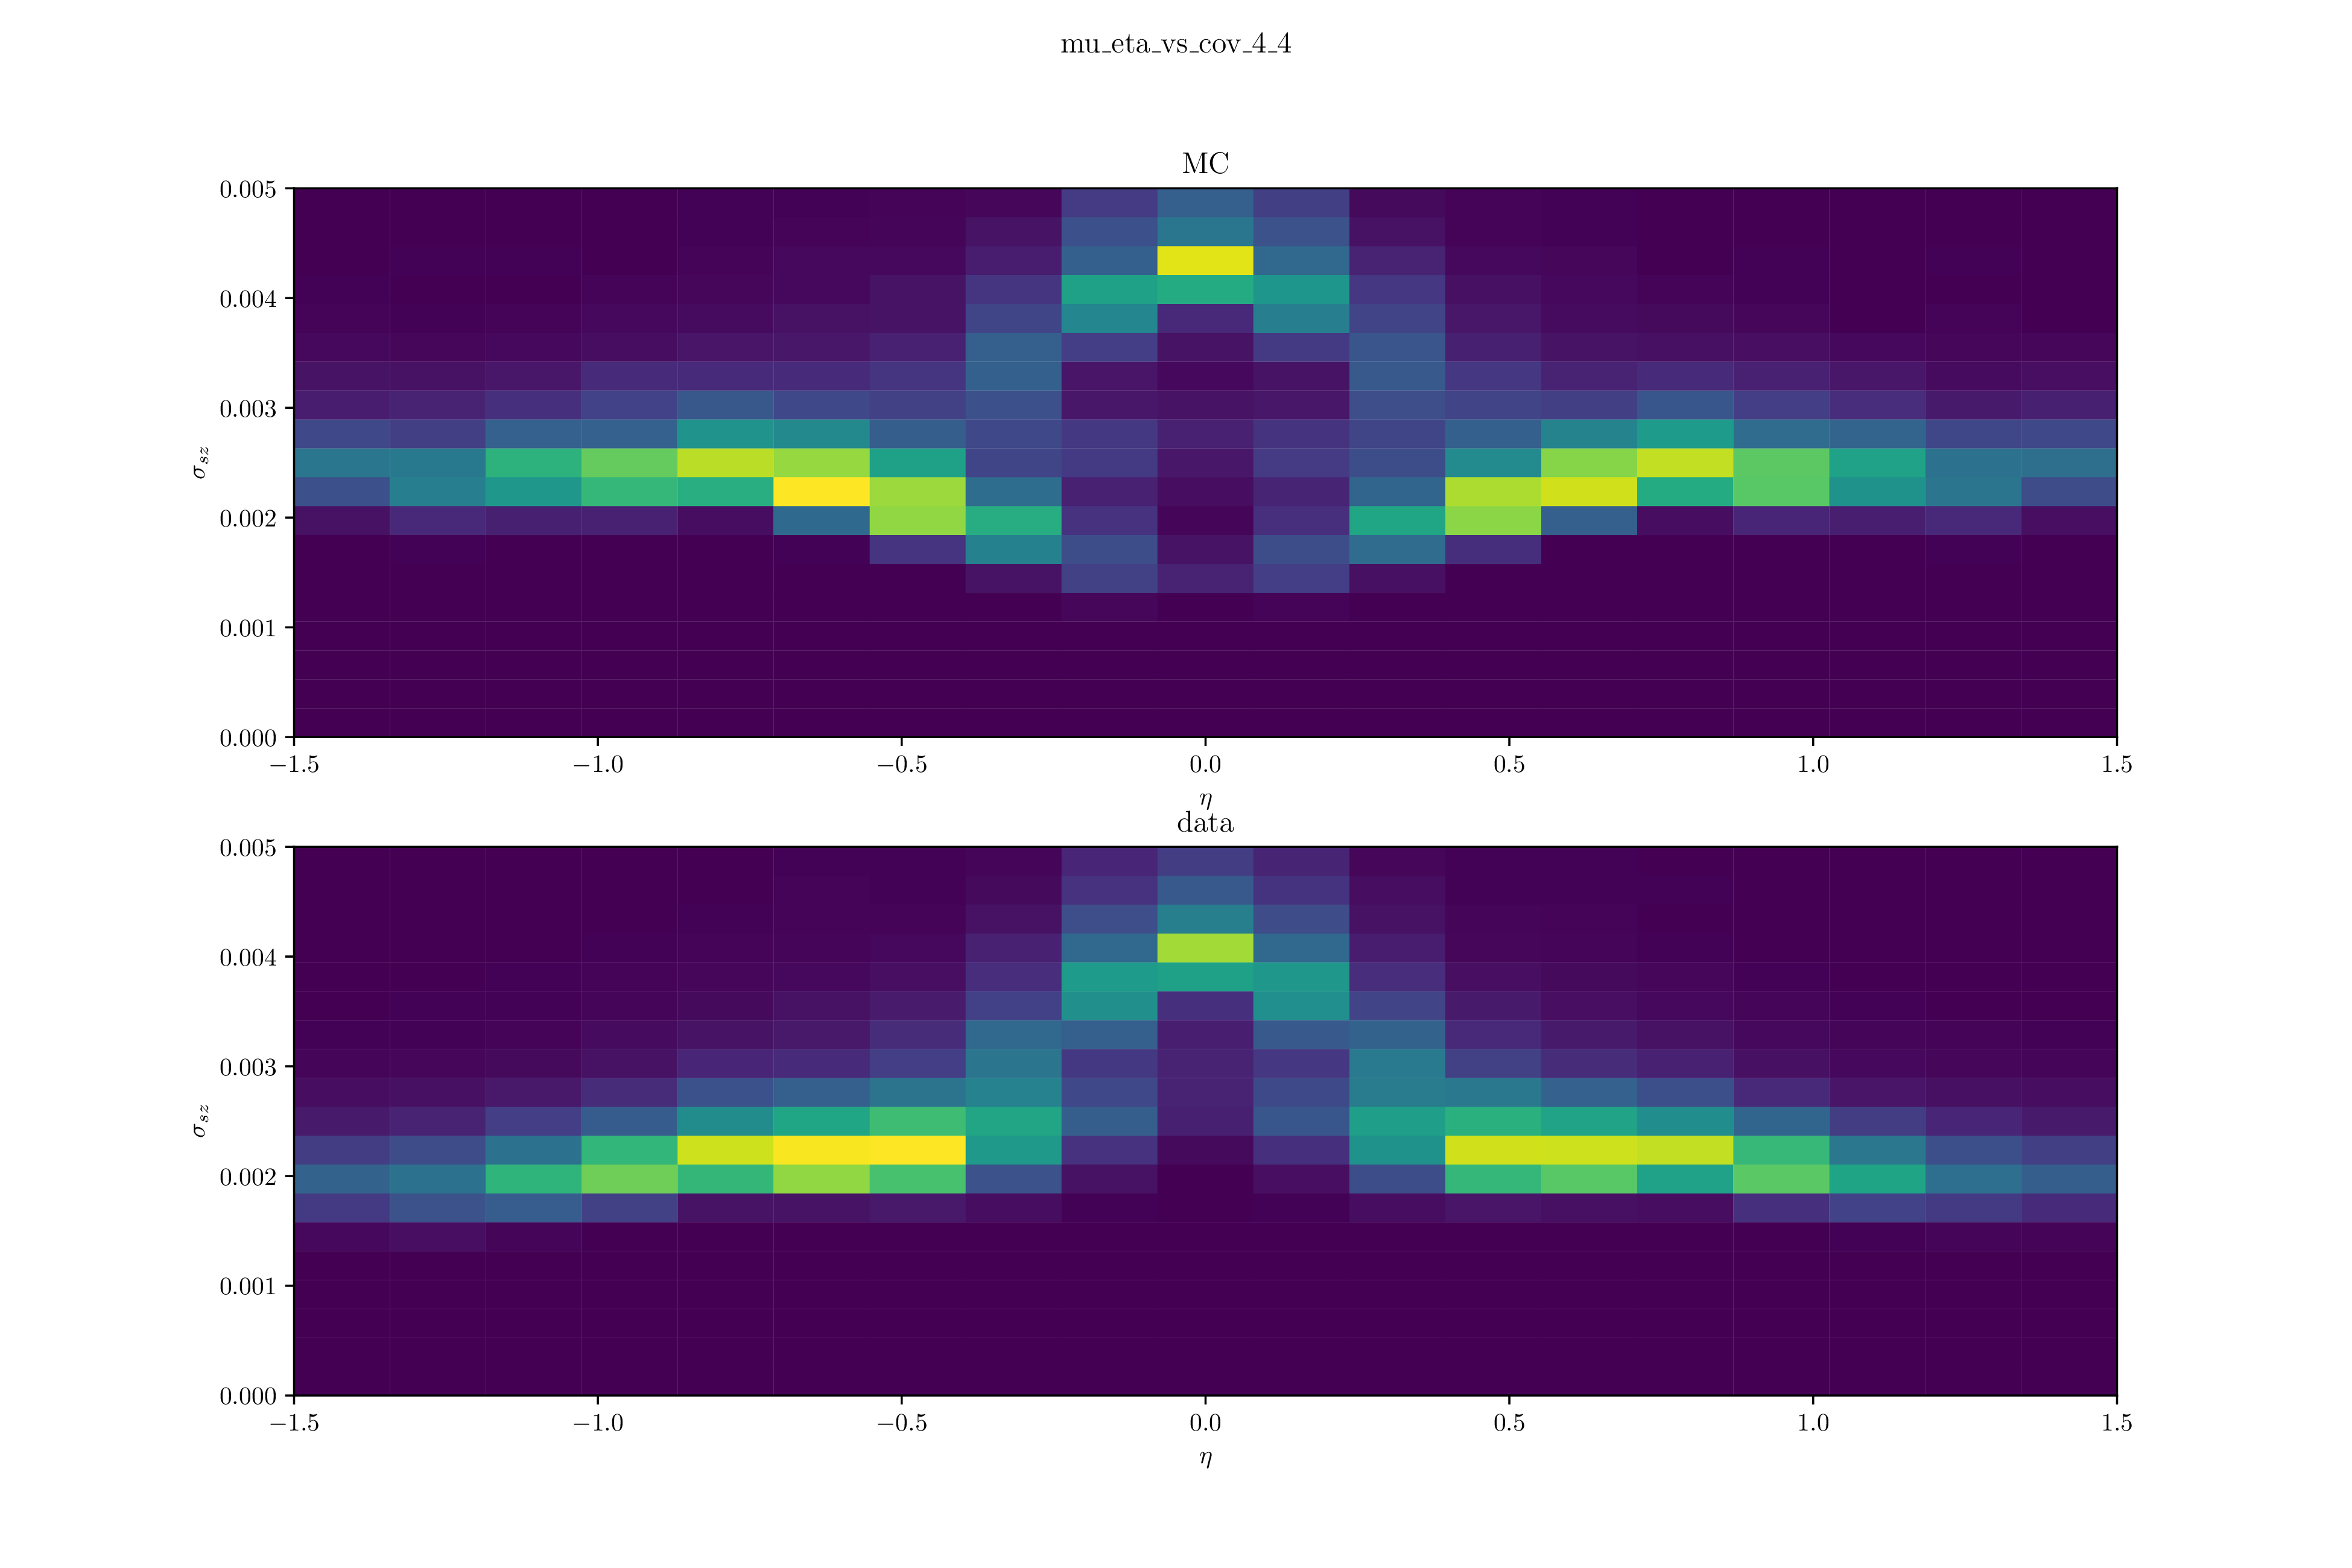
\includegraphics[width=\linewidth]{mu_eta_vs_cov_4_4.png}
\caption{2D histogram showing the 4th covariance matrix element of the muon as a function of $\eta$ for MC (top) and data (bottom). As you can see there is a distinctive feature in the barrel region for the MC which is not at all present in the data.}
\label{fig:mu-eta-vs-cov-4-4}
\end{figure}

These covariance matrix elements are extremely important for both the secondary
track fits and for the primary vertex fit. They are important for the secondary
track fits because the entire analysis relies on fitting these tracks within
the CMSSW framework which uses the covariance matrix when fitting multiple
tracks. Similarly, the primary vertex resolution is important as it is used to
compute the B direction when computing all of the final observables (missing
mass, etc.).

Fundamentally, I believe the current approach of trying to fix these issues
after the fact by applying corrections at the analysis level is wrong. Whatever
is causing these issues in the other matrix elements represents some
fundamental mismodelling of the detector in the Monte Carlo and because of the
complex nature of how these variables enter the analysis (through complex fits
of tracks) and so should be fixed at the simulation level and not papered over
after the fact.

\section{Primary Vertex Resolution}
As mentioned in the previous section, there are noticeable differences in the
covariance matrix between data and MC. In addition, there are obvious
differences in the primary vertex fit. If you look at the chi-squared and
number of degrees of freedom for this fit you find that these distributions do
not at all agree between data and MC, and this is important since the primary
vertex is used to compute all the final observables.

The current hypothesis is that these problems are caused by a mismodelling of
the radiation damage in the first pixel layer of the tracker. We have currently
tried to take this into account by adding a Gaussian smearing on the x, y, and
z coordinate of the primary vertex fit in MC. You can see that here:
\url{https://github.com/alatorre-caltech/BPH_RD_Analysis/blob/e9d8ac7ec8585be1badd68e43c1c48aa11751005/scripts/B2DstMu_skimCAND_v1.py#L268}.
Currently we actually apply a beamspot constraint at the ntuplization
level\footnote{Not clear if this is a good idea due to the fact that the
beamspot wandering is not actually simulated in MC.}, so that later we
primarily only have to apply a significant smearing in the z direction.

One current issue is that based on using the jacknife technique to estimate the
PV error, it appeared that we only needed to add an extra 5 $\mu m$ of
smearing. However, currently the fit wants to pull this closer to 15 $\mu m$.

The vertex resolution is extremely important, and in my opinion it is not the
correct approach to try to fix a mismodelling of the radiation damage in the
tracker by applying ad-hoc gaussian smearing after the fact. It clearly seems
to help the fit a lot, but it's unlikely that the complex effects of this
mismodelling cannot be captured with a simple gaussian smearing.

\section{Mismodelling in the Plus Minus Control Region}
It seems likely that there is at least one background in the control region
with two tracks that are oppositely charged that we are not currently modeling.
This is evident from two plots: the visible mass and the mass of the two extra
tracks.

\section{Beamspot Calibration}
The beamspot in all of the MC assumes the beam is travelling exactly in the
center of the CMS detector. However, in actual data the beamspot wanders
throughout a run. Furthermore, there are some differences in the beamspot shape
between data and MC (specifically, beamspot tilts are not simulated in MC). For
more information about this talk to Riccardo Manzoni.

Here, I think we never had the time to fully explore whether this was a
significant issue. There was a beamspot calibration weighting scheme created
(see
\url{https://github.com/alatorre-caltech/BPH_RD_Analysis/blob/master/analysis/beamSpotCalibration_v1.ipynb}),
however it seemed to be strongly correlated with the B pT calibration and it
was never clear whether it was actually doing what we thought and so was
abandoned.

\section{Smaller Issues}
There are a lot of smaller issues that need to be looked into once the larger issues like the covariance matrices and primary vertex resolution are solved. In this section I will describe these issues.
\subsection{Event Migration}
Originally in the Combine fit, there was no way for events to migrate between
control regions. This wasn't correct since when the systematic for the track
efficiency is moved that will cause events to migrate between control regions.
The correct way to do this is to take a given track efficiency curve and then
apply weights for that event to move between control regions. For example, if
an event ends up in the plus control region (one positive extra track) with an
extra track pT of 1 GeV, and then the systematic for the track efficiency at 1
GeV moves to 80\%, then the event should be given a weight of 80\% in the one
track control region and a weight of 20\% in the signal region.

However, to do this correctly would have been very difficult with the existing
structure of the fit. The two problems are that the events are stored in
different files and dataframes depending on whether they are signal or control
regions throughout the fit and second that the fit was only designed to give
each event a single weight (and not move them around). Therefore, a complex
approach that was hoped to capture most of the issues was implemented but which
is not quite right. In this case we duplicate all the events in the dataset
(necessary because the entire runCombine.py assumes events do not move) and
move them to the control region they would be if they dropped the lowest pt
extra track. In other words, for events in the PM control region, if the plus
track is the lowest pt, then it would be duplicated and the duplicate copy
would be put in the minus control region. Then we do apply the weights
procedure discussed previously but only for the extra track with the lowest pt.

This did improve the fit at the time, but it still fails to capture some
potentially important features. For example, if you have an event in the PM
control region and both tracks are very low energy, it is possible for that
event to end up in the signal region, but with the current scheme that is not
possible.

Although it would be a lot of work, I think it would be better to update
runCombine.py to not assume that all systematics are given by simple weights
and that some can be given by a rebinning of all the events. This was actually
partially implemented here:
\url{https://github.com/alatorre-caltech/BPH_RD_Analysis/blob/e9d8ac7ec8585be1badd68e43c1c48aa11751005/Combine/runCombine.py#L285}
for the PV resolution which cannot be done simply with weights since you are
adding random numbers to the primary vertex. But this partial implementation is
kind of ad-hoc and it might be better to simplify it.
\subsection{Correlation of Systematics}
There are a \emph{lot} of corrections applied to the MC to correct for various
data/MC disagreements. A partial list is here:
\begin{itemize}
\item Covariance matrix of all tracks
\item PV resolution
\item B pT weights
\item B eta weights
\item Additional track pT weights
\item Number of pileup tracks
\item Number of additional tracks from PV
\item Low pT track efficiency
\item Trigger scale factor weights
\item Muon ID scale factor weights
\end{itemize}
Although many of these are likely independent, some of them almost certainly
are not. For example the low pt track efficiency, the additional track pt
weights, and the PV resolution are all likely the result of a mismodelling of
the tracker.

Right now the fit assumes all the systematics are completely uncorrelated, but
since that's not true, these issues either need to be fixed upstream in the MC
so that the systematics are negligible or the correlation needs to be accounted
for in the fit.
\subsection{Random Tracks from the PV}
Currently the model for floating the number of additional tracks from the PV
assumes a Poisson distribution. However, this is not obvious whether it should
be and some preliminary checks suggest it is not. This should be modelled
correctly.
\subsection{Form Factors for $\mathrm{D}^{**}$ Decays}
Michele Papucci, the author of the Hammer library, created some code to
estimate form factor corrections for the doubly excited D states. However, this
code was never actually published in the repository and only existed in Olmo's
home directory, so I have not been running with these form factors in the fit.
When I last talked to Michele he was positive about publishing these so that
they could be used by anyone, but I haven't followed up on that.
\subsection{Central Values for Pulled Systematics}
For some backgrounds which aren't well known the fit may pull them by several
standard deviations. Since Combine does not actually know what happens beyond
$1\sigma$ (you only provide $+1\sigma$ and $-1\sigma$ histograms), these
systematics should be recomputed and you should give Combine the histogram for
whatever $\sigma$ it is currently fitting at. For example, if Combine wants to
pull some parameter to $+2\sigma$, we should instead provide $+2\sigma$ and
$-2\sigma$ histograms to Combine.
\end{document}
